\section{Creating the AST}
\subsection{Operators and rewrite rules}
As described in section \ref{sect:antlr:ast}, ANTLR provides operators and
rewrite rules for augmenting the grammar specification into generating a useable
AST. In many cases, it is a simple matter of defining which tokens to use as
root, and which to omit. This is done using the two basic operators \verb!hat!
(\^{}) and \verb!exclamation mark! (!). Figure \ref{code:ast:exoperator} shows an
example where the exclusion operator is used to exclude the superfluous brace
tokens from the AST in the \verb!ftWordsValue! production.

\begin{figure}[h]
\begin{verbatim}
ftWordsValue : literal | (LBRACESi! expr RBRACSi!);
\end{verbatim}
\caption[AST exclusion operator example]{Using the exclusion operator to exclude
the superfluous brace tokens from the AST, leaving only the expression subtree}
\label{code:ast:exoperator}
\end{figure}

Further the hat operator which is, as previously mentioned, used to promote
tokens to be roots in a subtree was utilized to augment certain expressions into
taking a natural hierarchial tree structure. Figure \ref{code:ast:hatoperator}
illustrates how not only how the hat operator is used to create subtrees from
expressions, but also how precedence is implicitly encoded into the grammar as
mentioned in section \ref{sect:xquery:precedence}.

\begin{figure}[h]
\begin{verbatim}
additiveExpr : multiplicativeExpr (
              (PLUSSi | MINUSSi)^ multiplicativeExpr)*;
  multiplicativeExpr : unionExpr (
                       (STARSi | DIV | IDIV | MOD)^ unionExpr)*;
    unionExpr : intersectExceptExpr (
                (UNION | PIPESi)^ intersectExceptExpr)*;
\end{verbatim}
\caption[AST root node promotion operator example]{Using the root node promotion
operator to define structuring of expressions such as arithmetic addition and set
operations}
\label{code:ast:hatoperator}
\end{figure}

This is behaviour is illustrated in figure \ref{tree:ast:arithmetic}, which is
the AST generated for the simple arithmetic expression \verb!1+2*3-2*15!.

\begin{figure}[h]
 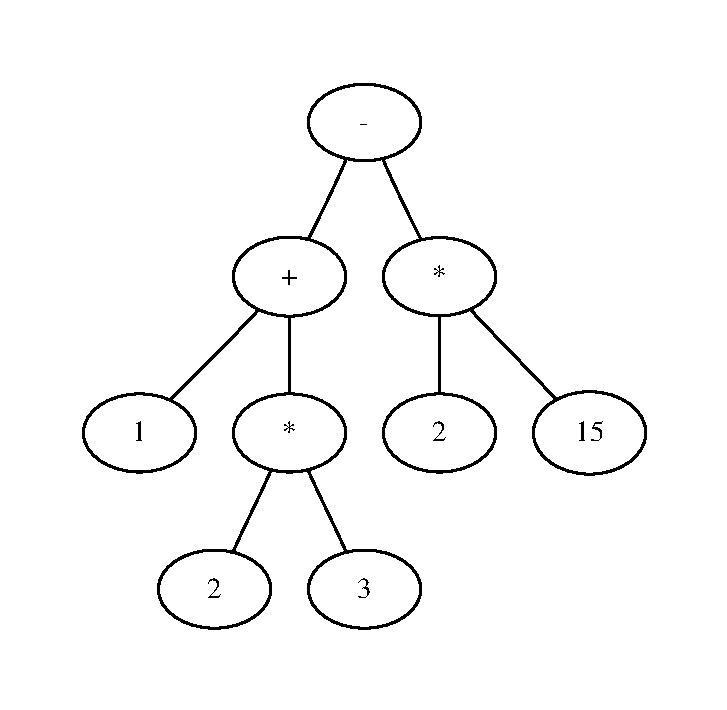
\includegraphics{img/graphs/arithmetic1}
\caption{Arithmetic AST example from the expression \texttt{1+2*3-2*15}}
\label{tree:ast:arithmetic}
\end{figure}

In addition to the operators, rewrite rules have been used in the the more
complex cases where simple operators were not sufficient. This is necessary in
the cases where it is impossible to simply exclude one token, typically in
productions that can produce lists. Figure \ref{code:ast:rewritelist}
illustrates an example for the \verb!letClause! production, where it is only
interesting to preserve the list of variable bindings, which can occur several
times.

\begin{figure}[h]
\begin{verbatim}
letClause : LET varBinding (COMMASi varBinding)*
            -> ^(AST_LETCLAUSE varBinding+);
\end{verbatim}
\caption[AST rewrite rule for the \texttt{letClause} production rule]{Using
rewrite rules to conserve only a list of variable bindings in the AST}
\label{code:ast:rewritelist}
\end{figure}

\subsection{FLWOR expressions}
FLWOR expressions are one of the more complex constructs in XQuery, and
naturally the AST will quickly become complex if care is not taken to include
only the necessary tokens and substrees to preserve information.

On the top level there is the \verb!flWORExpr! production rule, which a
composite of \verb!forClause!, \verb!letClause!, \verb!whereClause!, and
\verb!exprSingle!. Figure \ref{code:ast:flwor} shows the rewrite used for this
production. In this case, a subtree is generated with the imaginary token
\verb!AST_FLOWR! as root. The \$fc and \$lc variables are lists of
for-clauses and/or let-clauses. These are then followed by an optional
where-clause, and an optional orderby-clause. Finally the list of children in
this subtree is terminated by an \verb!exprSingle!, denoting the expression
after the RETURN token.

\begin{figure}[h]
\begin{verbatim}
fLWORExpr : (fc+=forClause | lc+=letClause)+ whereClause?
            orderByClause? RETURN exprSingle
    -> ^(AST_FLWOR $fc* $lc* whereClause? orderByClause? exprSingle);
\end{verbatim}
\caption{AST rewrite rule for FLWOR expressions}
\label{code:ast:flwor}
\end{figure}

In this example we have eliminated a redundant token (\verb!RETURN!) and
condensed the information in the production rule into a subtree more suitable
for traversion, data flow analysis and transformation.

Note however, that this structure is subject to change as requirements may 
emerge. This will be trivial since it is only necessary to edit the rewrite
rule, regenerate the parser, and recompile the program.

The for-clause uses the same technique for augmenting a list of tuplet
definitions, and the child production \verb!forClauseTupletDef! uses simple
operators to exclude superfluous tokens. These rules can be seen in figure
\ref{code:ast:forclause}. 

\begin{figure}[h]
\begin{verbatim} 
forClause : FOR forClauseTupletDef (COMMASi forClauseTupletDef)* 
            -> ^(AST_FORCLAUSE forClauseTupletDef+);

  forClauseTupletDef : DOLLARSi! varName typeDeclaration? positionalVar? 
                     ftScoreVar? IN! exprSingle;
\end{verbatim}
\caption{AST rewrite rule for for-clauses}
\label{code:ast:forclause}
\end{figure}

The let-clause was described earlier in this section, however note that the for-
and let-clauses can be mixed at free will in the FLWOR-expression, so thus
proper care must be taken when parsing the AST. Specifically, special conditions
will apply for determining the number of for- and let-clauses in the expression.
For example, it can be determined that there are no more for/let-clauses when
one encounters one of the following:
\begin{itemize}
  \item \verb!whereClause!
  \item \verb!orderByClause!
  \item \verb!exprSingle!
\end{itemize}

The optional where-clause is trivial. The rewrite rule adds an imaginary
token for clarity and omits the \verb!WHERE! token, as can seen in figure
\ref{code:ast:whereclause}.

\begin{figure}[h]
\begin{verbatim} 
whereClause : WHERE exprSingle
              -> ^(AST_WHERECLAUSE exprSingle);
\end{verbatim}
\caption{AST rewrite rule for where-clauses}
\label{code:ast:whereclause}
\end{figure}

The orderby-clause is also a trivial case. As with the where-clause, an
imaginary token is added for clarity, and the \verb!STABLE! token is preserved
if it is present in the input. In this case, an alternative solution would be to
flag the imaginary root node token as ``stable''. As described in section 
\ref{sect:antlr:ast}, this can be done by subclassing the \verb!CommonTree! (or
\verb!BaseTree!) classes and adding a custom tree adaptor to set such flags on
tokens. The rewrite rule for the orderby-clause is shown in figure
\ref{code:ast:orderbyclause}.

\begin{figure}[h]
\begin{verbatim} 
orderByClause : (ORDER BY | STABLE ORDER BY) orderSpecList
                -> ^(AST_ORDERBYCLAUSE STABLE? orderSpecList);
\end{verbatim}
\caption{AST rewrite rule for orderby-clauses}
\label{code:ast:orderbyclause}
\end{figure}

Finally, the \verb!exprSingle! rule terminates the FLWOR expression. This rule
isa placeholder for any valid expression, and thus it carries no meaning in
itself but rather in the sense of what is deduced from the input.

Figure \ref{tree:ast:flwor} shows the AST generated for the expression 

\begin{figure}[h]
 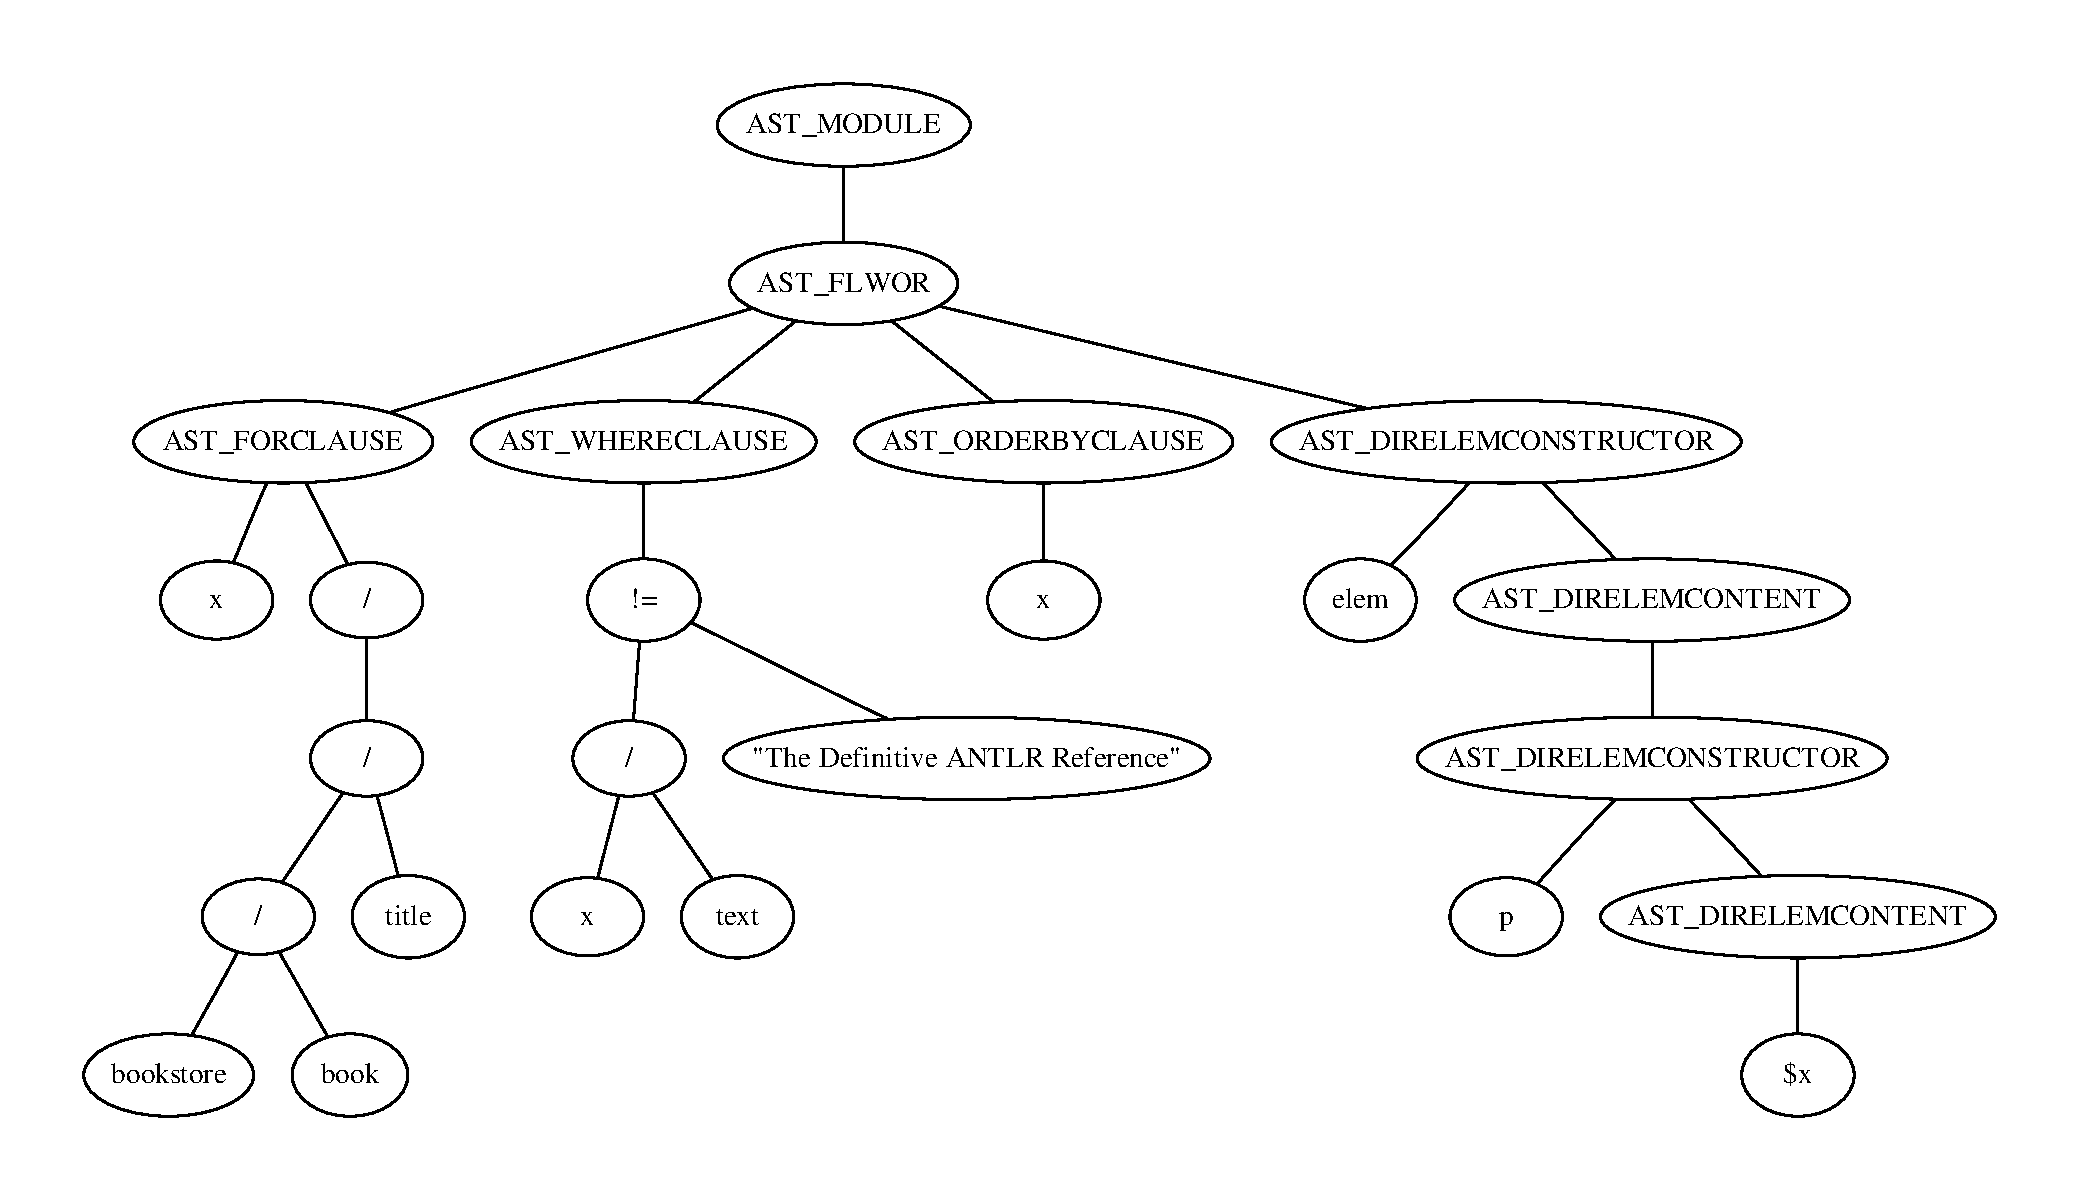
\includegraphics[width=1\textwidth]{img/graphs/flwor1}
\caption{Generated AST tree for a simple FLWOR-expression}
\label{tree:ast:flwor}
\end{figure}

\subsection{Path expressions}
\subsection{Function declarations}